\documentclass{article}
\usepackage{amsmath}
\usepackage{amssymb}
\usepackage{graphicx}
\usepackage{hyperref}
\usepackage[version=4]{mhchem}

\title{Example 6}
\date{}

\begin{document}
\maketitle

In \(\triangle A B C, A D\) is the median. \(B E\) and \(A C\) meet at \(E . B E\) and \(A D\) meet at \(F\). If \(A E=E F\), show that \(A C=B F\).

Proof:
Extend \(A D\) to \(H\) such that \(D H=A D\).\\
\centering
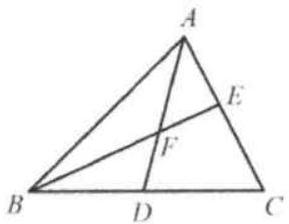
\includegraphics[width=\textwidth]{images/problem_image_1.jpg}

Since \(B D=C D\) and \(\angle B D H=\angle A D C\), then \(\triangle A C D \cong \triangle H B D\), \(A C=B H\), and \(\angle D A C=\angle H=\alpha\).

We are given that \(A E=E F\), so \(\angle A F E=\angle E A F=\angle B F H=\alpha\). Therefore in \(\triangle B F H, B F=B H=A C\).\\
\centering
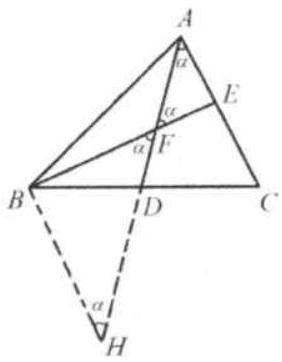
\includegraphics[width=\textwidth]{images/reasoning_image_1.jpg}


\end{document}
